
\begin{figure}[htbp]
\centering
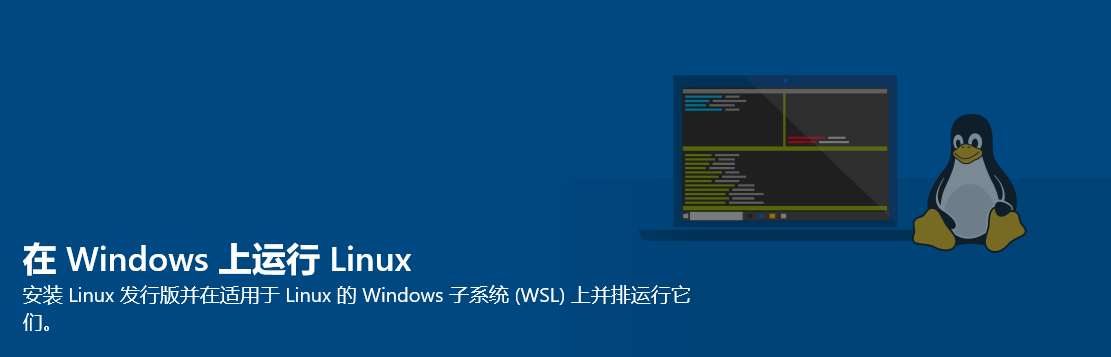
\includegraphics[width=0.7\textwidth]{docs/intro/images/WSL1.png} 
\caption{头图}
\end{figure}

\hr

\subsection{0x01 引言}

众所周知,尽管现在大部分学校的竞赛练习环境都是构建 XP 等 Windows 系操作系统,但是在 NOI 系列赛中,早已用上了 NOI Linux 这个 Ubuntu 操作系统的阉割版。  

\begin{figure}[htbp]
\centering
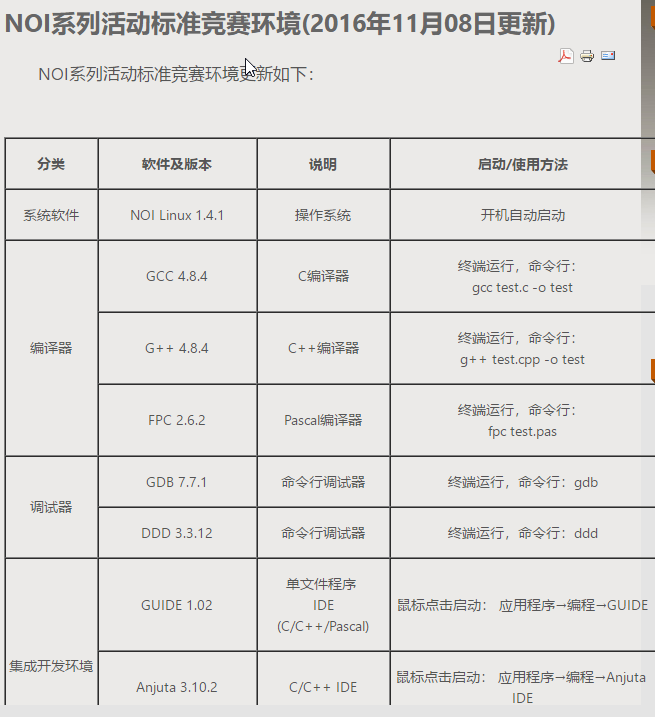
\includegraphics[width=0.7\textwidth]{docs/intro/images/WSL2.png} 
\caption{NOI 竞赛的环境要求}
\end{figure}           



或许大家对自己 Windows 环境下的 Dev-C++ 等都已熟识,但是当场景突然切换到 Linux 的时候,你会不会不知所措?

\begin{QUOTE}{}{}
「想用 Ctrl+C 复制,结果退出了程序」  



「平时 AC 的程序模板到了 Linux 上就 WA」……
\end{QUOTE}

\begin{figure}[htbp]
\centering
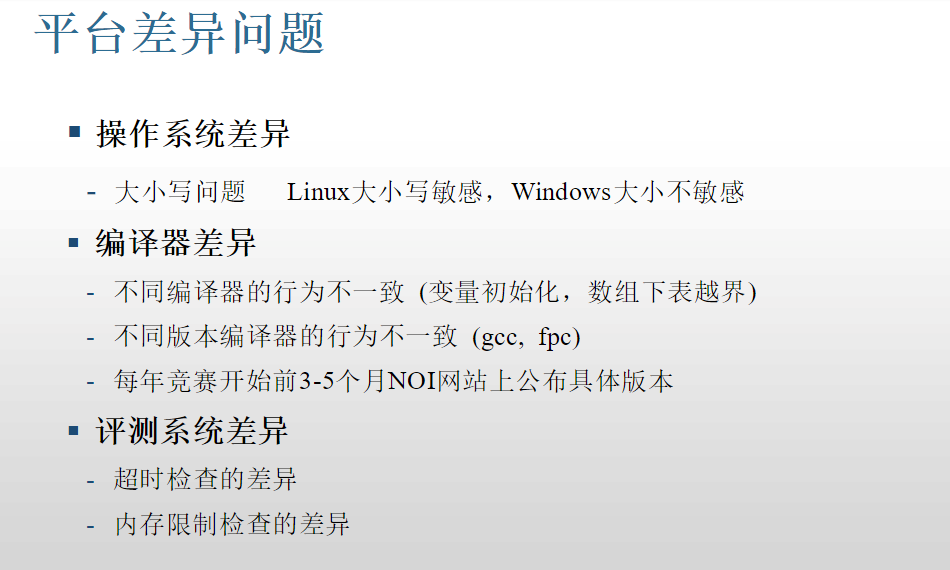
\includegraphics[width=0.7\textwidth]{docs/intro/images/WSL3.png} 
\caption{平台差异(转自百度文库”NOIP 标准评测系统及相关问题 “)}
\end{figure}



虽然在 NOI 的官网已经放出了 NOI Linux 的 ISO 镜像,但是如果跑虚拟机的话,配置也相当麻烦,包括激活 VMware,用 VMware 装系统开虚拟机等步骤,且 NOI Linux 默认自带图形界面,两个系统一起运行是低配党的噩梦。

Windows 10 作为微软的新一代操作系统,紧跟时代潮流,在一周年更新时推出了 Linux 子系统(WSL),可以供装不起 VMware 等虚拟机的同学食用。  

缺点是没有 NOI 评测用的 \textbf{Arbiter},但是在各大 OJ 背书的情况下谁在乎呢……

\begin{NOTE}{补充资料:何为 Linux 子系统(WSL)?(via 百度百科)}{}
 Windows Subsystem for Linux(简称 WSL)是一个为在 Windows 10 上能够原生运行 Linux 二进制可执行文件(ELF 格式)的兼容层。它是由微软与 Canonical 公司合作开发,目标是使纯正的 Ubuntu, OpenSUSE, Kali Linux 和 Debian 映像能下载和解压到用户的本地计算机,并且映像内的工具和实用工具能在此子系统上原生运行。  
 WSL 提供了一个微软开发的 Linux 兼容内核接口(不包含 Linux 代码),来自 Linux 的用户模式二进制文件在其上运行。  
 此子系统起源于命运多舛的 Astoria 项目,其目的是允许 Android 应用运行在 Windows 10 Mobile 上。此功能组件从 Windows 10 Insider Preview build 14316 开始可用。

\end{NOTE}


\hr

\subsection{0x02 准备}

首先,你需要一个最新的 Windows 10 操作系统,这点不必多说。  

其次,你需要配置一下开发人员模式环境。

\begin{enumerate}
\item 设置 -> 更新与安全 -> 开发人员模式框选 -> 是
\begin{figure}[htbp]
\centering
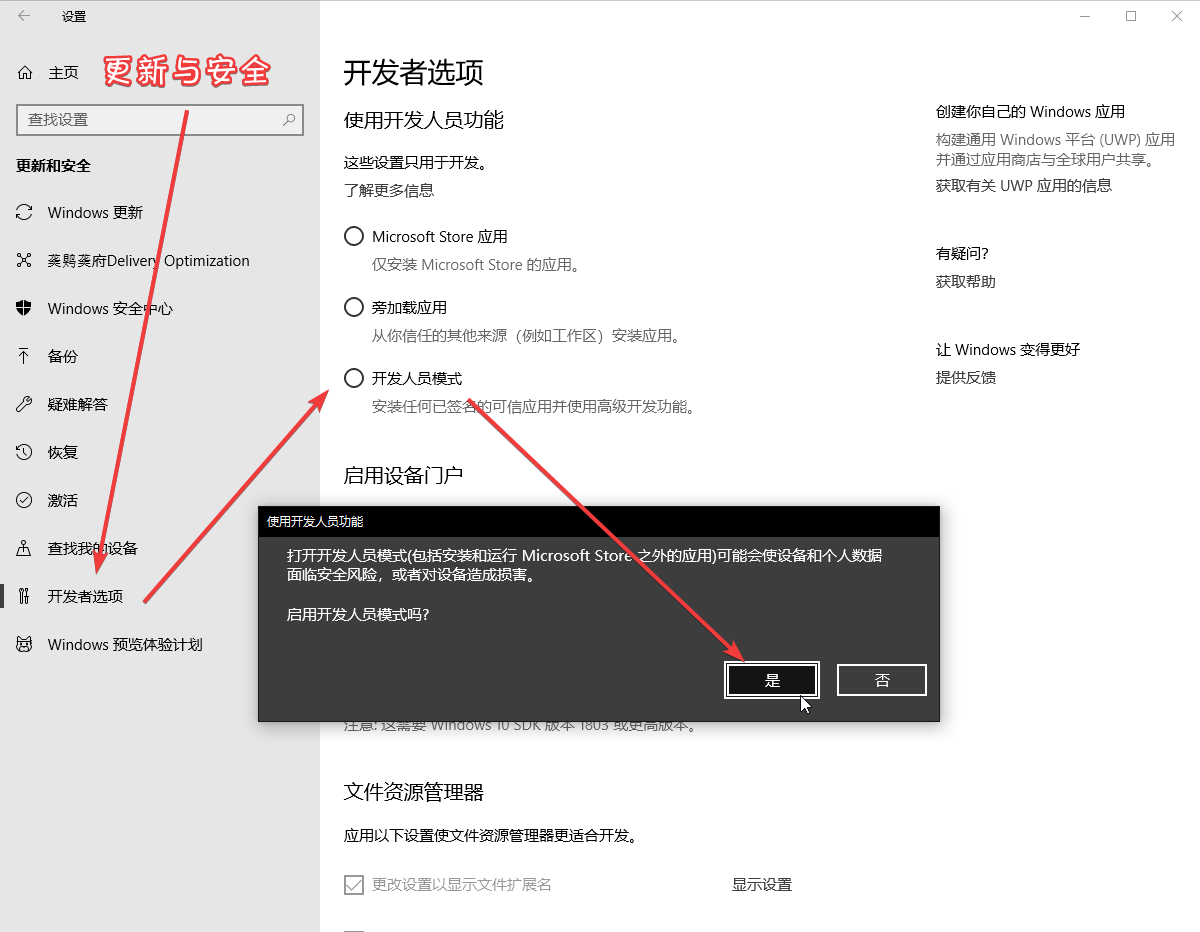
\includegraphics[width=0.7\textwidth]{docs/intro/images/WSL4.png} 
\caption{来,跟着箭头走}
\end{figure}     
\end{enumerate}



\textbf{Linux 区分大小写!}

\begin{figure}[htbp]
\centering
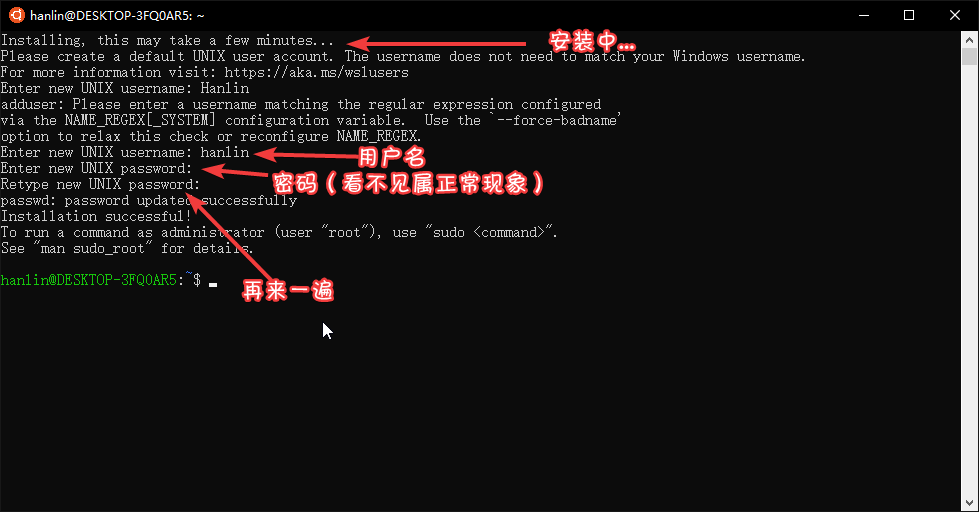
\includegraphics[width=0.7\textwidth]{docs/intro/images/WSL6.png} 

\end{figure}

 这样之后,一个纯净的 Ubuntu 系统安装完成了!

\subsection{0x04 基础配置}

 \textbf{ 以下命令均可直接右键复制粘贴进窗口哦!}

\begin{figure}[htbp]
\centering
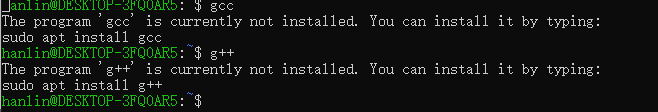
\includegraphics[width=0.7\textwidth]{docs/intro/images/WSL7.png} 

\end{figure}

 正如图片所示,这个系统纯净到连个编译器都没有,所以这一节来看看基础的环境配置。

\subsubsection{更换为国内软件源}

Ubuntu 默认的软件源在国外,我们可以换为国内的加快速度,如 \href{https://mirrors.tuna.tsinghua.edu.cn/help/ubuntu/}{清华 TUNA 的软件源}。  

可以访问 \href{https://mirrors.tuna.tsinghua.edu.cn/help/ubuntu/}{TUNA 的页面} 来获得国内源的信息。

\begin{WARNING}{}{}
 请在页面中寻找与自己系统版本相配的源(可使用 \texttt{sudo lsb\_release -a} 查看,具体详见 \texttt{0x03} )  
 除非你知道你在做什么,否则不要使用与自己的系统版本不匹配的源!     

\end{WARNING}


使用的命令

\begin{minted}{bash}
sudo cp /etc/apt/sources.list /etc/apt/sources.list.bak
sudo vim /etc/apt/sources.list
# (按 i 之后将上文的源右键粘贴进去,编辑完后按 Esc,再输入 :wq 和回车)
sudo apt update
sudo apt upgrade -y
\end{minted}

\begin{figure}[htbp]
\centering
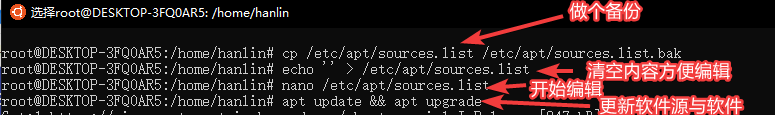
\includegraphics[width=0.7\textwidth]{docs/intro/images/WSL9.png} 

\end{figure}

\subsubsection{安装中文环境}

\begin{minted}{bash}
sudo apt install  language-pack-zh-han* -y
sudo locale-gen zh_CN.GB18030 && sudo locale-gen zh_CN.GB2312 && sudo locale-gen zh_CN.UTF8
# 中文字体,别忘了同意 EULA
sudo apt install fontconfig -y
sudo apt install ttf-mscorefonts-installer -y
# 下面的再执行一遍以防万一
sudo apt install -y --force-yes --no-install-recommends fonts-wqy-microhei
sudo apt install -y --force-yes --no-install-recommends ttf-wqy-zenhei
sudo dpkg-reconfigure locales
\end{minted}

使用 \texttt{sudo dpkg-reconfigure locales} 进入菜单,按空格选择带 \texttt{zh\_CN} 的选项,选完后回车,下一个菜单中选 \texttt{zh\_CN.UTF-8} 打回车。

\begin{figure}[htbp]
\centering
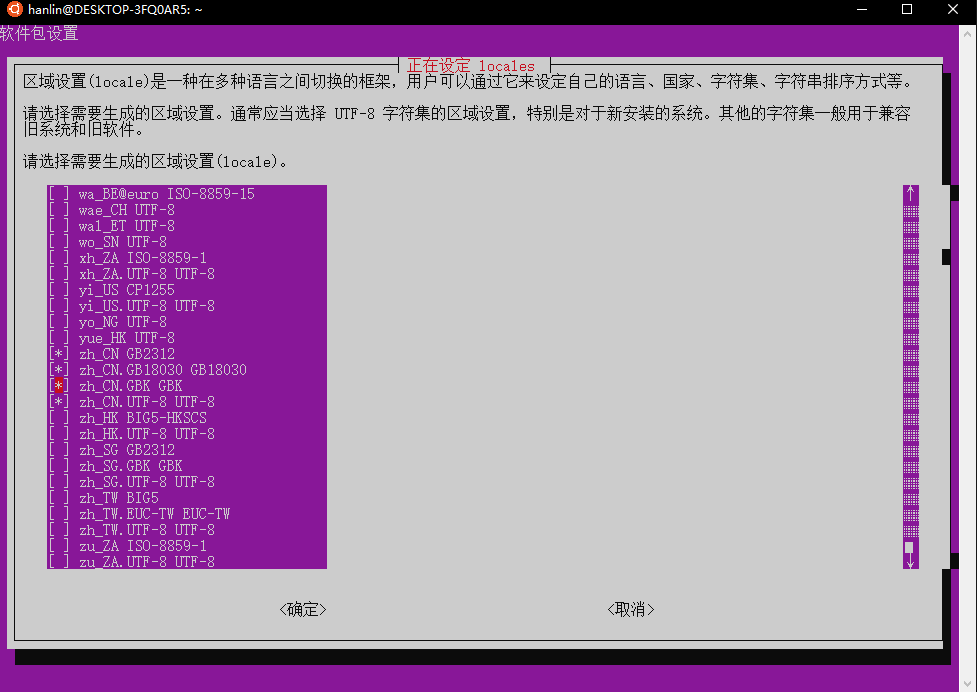
\includegraphics[width=0.7\textwidth]{docs/intro/images/WSL10.png} 

\end{figure}

\begin{figure}[htbp]
\centering
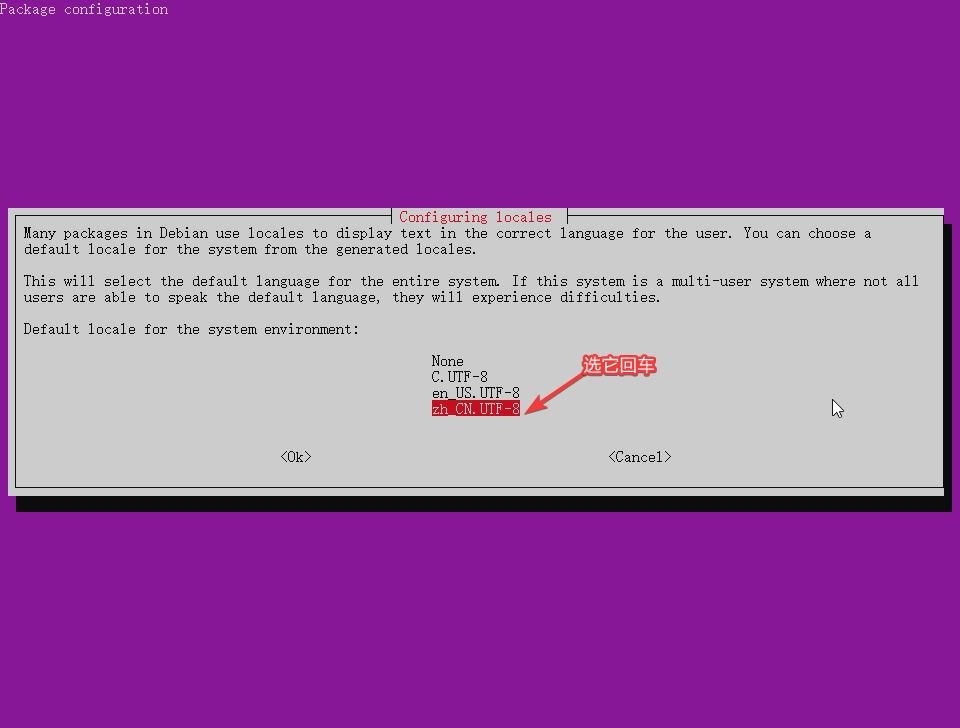
\includegraphics[width=0.7\textwidth]{docs/intro/images/WSL11.png} 

\end{figure}

 之后关上 Ubuntu 重开一遍登录,是不是变中文了?

再依次输入下列命令,把 \texttt{man} 帮助页替换为中文:\href{https://blog.csdn.net/qq_14989227/article/details/72954523}{via}

\begin{minted}{bash}
sudo apt install manpages-zh
sudo vi /etc/manpath.config
:1,$s#/usr/share/man#/usr/share/man/zh_CN#g
:wq
\end{minted}

 可以用 \texttt{man help} 测试下。

\subsubsection{安装编译环境}

\begin{minted}{bash}
sudo apt install build-essential vim ddd gdb fpc emacs gedit anjuta lazarus -y
wget http://download.noi.cn/T/noi/GUIDE-1.0.2-ubuntu.tar
tar -xvf GUIDE-1.0.2-ubuntu.tar
cd GUIDE-1.0.2-ubuntu
chmod +x install.sh && ./install.sh
\end{minted}

这是基础的 + NOI 官方要求环境,如有需要可以用 \texttt{apt install 程序名} 来安装别的。

若想安装其他版本可以参考下 \href{https://www.cnblogs.com/EasonJim/p/7144017.html}{这个}

来个程序玩玩:

\begin{minted}{bash}
$ vim cpuid.cpp
$ g++ -Wall cpuid.cpp -o cpuid
$ ./cpuid
AMD Ryzen 5 1400 Quad-Core Processor
\end{minted}

\textbf{Tips:Linux 环境下可执行文件可不带扩展名,实现方式看上方命令行 }

\subsection{0x05 进阶操作}

\subsubsection{安装图形环境,并使用远程桌面连接}

推荐图形环境用 xfce4,不臃肿。

\begin{minted}{bash}
sudo apt install xfce4 tightvncserver -y
# 或使用 sudo apt install xubuntu-desktop -y
# xubuntu 安装的软件多,基础环境可用第一种
\end{minted}

图形环境是个大头,因此要多等会,静静等待下载解包。

下面配置 xrdp:

\begin{minted}{bash}
sudo apt install xrdp -y
echo "xfce4-session" >~/.xsession
sudo service xrdp restart
\end{minted}

 为了防止和你计算机本来带的远程桌面冲突,最好换一下端口。

\begin{figure}[htbp]
\centering
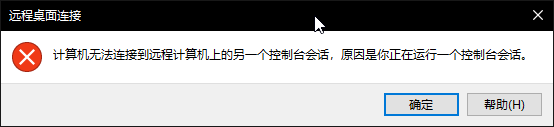
\includegraphics[width=0.7\textwidth]{docs/intro/images/WSL12.png} 

\end{figure}



\begin{enumerate}
\item \href{https://wenku.baidu.com/view/8246d96cdd36a32d72758143.html}{NOIP 标准评测系统及相关问题, smart0326, 2014-05-19, 百度文库}         
\item \href{https://baike.baidu.com/item/wsl/20359185}{WSL, 百度百科}        
\item \href{https://blogs.windows.com/buildingapps/2016/03/30/run-bash-on-ubuntu-on-windows/#cie8WdR3uSjgR5Ru.97}{Run Bash on Ubuntu on Windows, Mike Harsh, 2016-05-30, Windows Blog}         
\item \href{https://docs.microsoft.com/zh-cn/windows/wsl/about}{Windows Subsystem for Linux Documentation, MSDN}      
\item \href{http://www.noi.cn/2016-11-08-03-42-01}{NOI 系列活动标准竞赛环境, 2016-11-08, NOI 官网}      
\item \href{https://www.microsoft.com/zh-cn/p/ubuntu/9nblggh4msv6}{购买 Ubuntu, Microsoft Store}      
\item \href{https://mirrors.tuna.tsinghua.edu.cn/help/ubuntu/}{Ubuntu 镜像使用帮助, 清华 TUNA}      
\item \href{https://blog.csdn.net/qq_14989227/article/details/72954523}{Ubuntu 的 man 命令帮助如何设置中文版, Frank 看庐山, 2017-06-09}      
\item \href{https://sourceforge.net/projects/xming/}{Xming X Server for Windows, SourceForge}       
\item \href{https://zh.wikipedia.org/wiki/Sudo}{Sudo, Wikipedia}       
\end{enumerate}

\subsection{0x09 延伸内容}

\href{https://spencerwoo.com/dowww/}{Dev on Windows with WSL(在 Windows 上用 WSL 优雅开发)}

\subsubsection{后记}

本文最初发布于 \href{https://www.luogu.org/discuss/show/48491}{洛谷日报 \textbackslash{}\#6},现由原作者搬运至此,有删改。      
